\section{Motion Control}
Motivation, General idea, terminology, 
\subsection{Space Time Constraint}
\subsection{Optimal Control}
\subsection{Reinforcement Learning}

\subsubsection{Markov Decision Process}
We formulate the bicycle control problem as a POMDP. A Markov decision process (MDP) is a tuple $(S, A, R, D, P_{sas'}, \gamma)$, where $S$ is the \emph{state} space; $A$ is the \emph{action} space; $R$ is the \emph{reward function}; $D$ is the distribution of the initial state $s_0$; $P_{sas'}$ is the transition probability; and $\gamma \in [0, 1]$ is the discount factor. For example, in the bicycle balance task, we choose the state space $S$ to include the tilt angle of the bike, the tilting speed and the handlebar angle. We choose the action $A$ to be turning the handlebar at a certain speed. We choose the reward function $R$ at the state $s$ to be
\begin{equation}
\begin{array}{ll}
R(s) = & \left\{ \begin{array}{ll}
1 & \textrm{if the bicycle remains upright,}\\
0 & \textrm{otherwise.}
\end{array} \right. \\
\end{array}
\label{eq:balanceReward}
\end{equation}
The initial state $s_0$ is drawn from a random perturbation near the upright orientation of the bicycle. The state transition is calculated using simulation, and we do not discount the rewards ($\gamma = 1$).

A \emph{policy} is a mapping from states to actions: $\pi : S \mapsto A$. The \emph{return} of a policy is the accumulated rewards along the state trajectory starting at $s_0$ by following the policy $\pi$ for $N$ steps.
\begin{displaymath}
V^\pi(s_0)=\sum_{i=0}^N{R(s_i)}
\end{displaymath}
The \emph{value} of a policy is the expected return with respect to the random initial state $s_0$ drawn from D.
\begin{equation}
V(\pi)=E_{s_0\sim D}[V^\pi(s_0)]
\label{eq:policyValue}
\end{equation}
The optimal solution of an MDP is the policy that has the maximum value $\pi^*=\arg\max_\pi V(\pi)$. The optimal policy in the bicycle balance example decides how to turn the handlebar under different situations so that the bicycle can stay upright for the longest time.

Our MDP is partially observable because we choose to observe only a selected subset of all the simulation states. We have found that focusing on a small number of relevant states for each task results in a more efficient learning process. The actions are also selected based on our prior knowledge of the task. Table~\ref{table:states} and~\ref{table:actions} summarize all the states and actions used across our different examples. The 25 states in Table~\ref{table:states} may seem exhaustive, but we only use a subset of them (typically not more than eight states) for each task.


\subsubsection{Policy Search}
We apply policy search to optimize the control policies. Unlike value iteration, policy search can be easily applied to MDPs in high dimension and with continuous state and action spaces. This algorithm searches for the optimal policy within a parameterized functional space $\pi^*\in\Pi$. During policy search, one or more random policies are generated as an initial guess. These candidates are evaluated and improved iteratively. Policy improvement can be guided using the policy gradient \cite{Ng:2000:PPS}, trajectory optimization \cite{Levine2013} or other optimization techniques \cite{Heidrich-Meisner:2008}. Policy search ends when the iteration converges or the maximum number of iterations is reached.


\paragraph{Policy Parametrization}
\label{sec:parametrization}

\begin{figure}[!t]
  \centering
  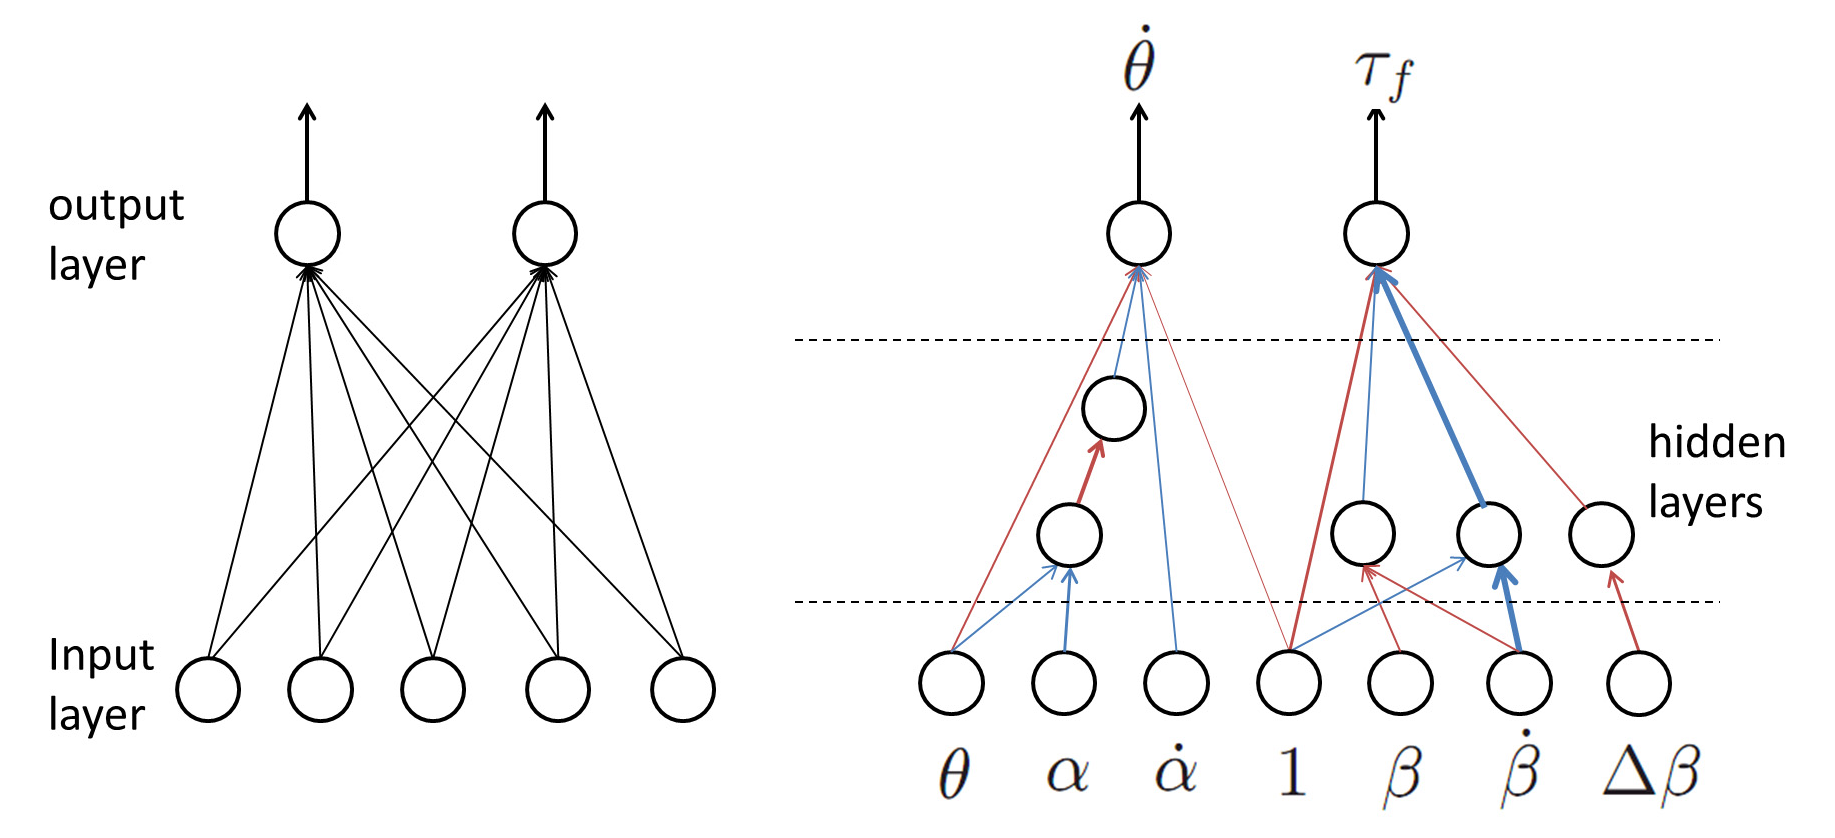
\includegraphics[width=3.4in]{figures/simpleNetwork}
  \caption{Left: A simple neural network with input and output layers that are directly connected. Right: A neural network learned using our algorithm for balancing on the front wheel. Blue arrows mean negative weights while red mean positive weights. The width of the arrows encodes the magnitude of the weights. }
  \label{fig:simpleNetwork}
\end{figure}

We use two types of parametrizations for the bicycle control problem: splines for feed-forward control and neural networks for feedback control. We found that most of the stunts can be categorized into momentum-driven, balance-driven or a combination of the two. The momentum-driven stunts involve vigorous full body motions to manipulate the bicycle to a desired orientation. Coordinated full body motions with large magnitude are essential, but the short duration of this type of stunts makes balance easy to maintain. For this reason, we use feed-forward controllers and represent the action trajectories as cubic Hermite splines. Assuming that the number of control points is given, the parameters to optimize are the time and the value of the control points\footnote{We do not optimize the tangents at the control points and we set them to be zero.}.

Balance-driven stunts require that the rider carefully adjusts his or her COM and maintains a stunt pose for a longer period of time. Feedback balance control is vital to the duration of the performance, which determines the success or failure of the stunt. We use neural networks for their ability to approximate a wide range of functions. The inputs to a network are the observed states, and the outputs are the actions. Figure~\ref{fig:simpleNetwork} Left illustrates a simple neural network that directly connects the input and the output layers. The output of neuron $i$ is
\begin{displaymath}
v_i=\sigma(\sum_j w_{ij} v_j)
\end{displaymath}
where $w_{ij}$ is the connection weight between neuron $i$ and $j$, and $\sigma$ is the sigmoid function $\sigma(x) = 1/(1+e^{-x})$.

Parametrization determines the potential quality of the optimal policy. The network shown in Figure~\ref{fig:simpleNetwork} Left is too simple for representing a complex policy required by bicycle stunts. However, it is not clear how to manually design the network structure, given the control policies of unsuccessful stunts. For this reason, we use NEAT to search for both the structure of the neural network and its weights simultaneously, which finds far better policies than searching over a fixed network. Figure~\ref{fig:simpleNetwork} Right demonstrates the learned network for the balance task of a bicycle endo using NEAT. See Chapter~\ref{sec:improvement} for more details.

\paragraph{Policy Evaluation}
To evaluate a policy, we formulate a reward function in the following form:
\begin{equation}
R(s)=R_t(s)+wR_r(s)
\end{equation}
where $R_t$ and $R_r$ are task-specific and regularization terms respectively. $w$ is the weight.

We use eq.(\ref{eq:balanceReward}) as the task-specific reward for balance-driven tasks. As the reward is accumulated over time, the return counts the number of frames that the bicycle stays upright. The task-specific reward varies for each momentum-driven stunt. For example, the reward for initiating an endo (lifting the rear wheel) is to maximize the negative pitch angle of the bike $R_t=-\beta$. We refer the readers to Chapter \ref{sec:results} and for more detailed descriptions of task-specific rewards.

Given the task-specific reward term alone, multiple optimal policies could exist. Taking the balance task as an example, a policy that rides in a straight line and another that oscillates in a sinusoidal path by periodically swinging the handlebar can both balance well and thus yield the same value. The regularization term is mainly used to eliminate this ambiguity. We use the regularization term $R_r=\frac{1}{|\theta|+\epsilon}$ to express our preference of riding straight. In our examples, all the regularizers are in the form of
\begin{displaymath}
R_r = \frac{1}{|X|+\epsilon}
\end{displaymath}
where $X$ can be substituted by $\alpha$ for the upright bicycle position, $\Delta \theta$ for the desired steering angle, $\Delta \beta$ for the desired pitch angle, $\Delta v$ for the desired speed, $(x, y, z)$ and $(\phi, \psi, \chi)$ for small changes of rider's pelvis position and torso orientation. A small number $\epsilon$ in the denominator is used to bound the reward.

We do not explicitly minimize the rider's effort in the reward function because it is difficult to balance the effort minimization objective and the task-specific objective for difficult stunt actions. However, we limit the maximum actuated joint torques of the rider in the simulation to ensure that the rider does not possess super-human strength.

We run multiple simulations with different initial configurations $s_0$, which are sampled from random perturbations of the default bicycle velocity and orientation, to evaluate the value of a policy. At each simulation step, our algorithm calculates the reward for the current state, and accumulates this until the bicycle falls or after 1000 time steps. The average return of all the simulations is the value of the policy.

\paragraph{Policy Improvement}
\label{sec:improvement}

Many policy improvement methods utilize the policy gradient \cite{Peters:2008} to perform iterative ascending operations. However, our simulation of bicycle stunts involves frequent discrete events such as establishing and breaking contact, which invalidates the gradient information. For this reason, we use sample-based stochastic optimization techniques. We apply CMA to search for the feed-forward controllers since the parametrization of splines is fixed. We use NEAT to search for feedback controllers, including the structure and the weights of the neural network. NEAT has many similarities to genetic algorithms, but it is tailored to the creation of neural networks. We will describe NEAT briefly below. For further details we refer readers to the original paper \cite{Stanley:2002:ENN}.

NEAT iteratively performs evaluation, selection, crossover and mutation. To maximize the value of a policy, NEAT starts with a simple network structure, in which the input and the output layers are directly connected. A population of such networks with random weights is drawn as an initial guess. These candidate policies are evaluated and the top 20\% are selected to survive. Pairs of randomly-selected surviving policies are crossed over to produce a new generation (more on this below). Mutations (with low probability) can perturb connection weights, add a neuron or add a connection. Note that the addition of a neuron or a connection complexifies the network structure and enriches the class of functions that it can represent.

Crossover is nontrivial in NEAT because the parent neural networks can have different topologies. To overcome this difficulty, the newly-added neuron or connection is assigned a unique innovation number, which tells the history of the mutation and how to match up neurons or connections between parents during crossover. The neurons or connections that share the same innovation number across parents are from the same ancestor, which will be inherited randomly by the child sample. The neurons or connections that have no counterparts in the other parent are from different mutations. They will be inherited from the parent with the higher value.

The evolution ends when the policy values do not increase over a certain number of iterations or the maximum number of iterations is reached.
